\capitulo{5}{Aspectos relevantes del desarrollo del proyecto}

En este apartado se recogen los aspectos más importantes o relevantes del desarrollo del proyecto. Desde las decisiones tomadas y las implicaciones que conlleva. Además de los problemas que fueron surgiendo.

\section{Comienzo del trabajo final de grado}
La idea de mi proyecto, surge de la noche a al mañana, porque el problema es que era 20 de Julio y no tenía nada que entregar, ya que iba a hacer otro proyecto en Knime, dejándolo para otro curso. 

Pero no podía dejar pasar una oportunidad. Fue más una falta de motivación y de malas sensaciones que otra cosa.

Por lo que me decidí estudiar como estaba el mercado de la programación móvil, descubriendo Flutter. Me gustó mucho, todo lo que se comentaba sobre este \emph{Framework}, eran cosas buenas, que era algo nuevo y sobretodo lo que más me decidió a cogerlo, es el respaldo que le daba Google.

Esto se lo comenté a mis tutores de trabajo final de grado, dándome el visto bueno, pero que tenía que trabajar mucho, para llegar a la calidad esperada. Por lo que era un reto enorme al que me enfrentaba, pero como digo, no se pueden dejar pasar las oportunidades, además que por otra parte lo que más me incentivaba, es a la hora de buscar trabajo, no decir que solo me quedaba el TFG. 

Ya que muchas de las empresas me decían que me esperaban a que terminase, para luego cogerme. Y yo no podía esperar, porque si no hacía el TFG, debía de trabajar para no tener que pensar en esto. Por lo que me encontraba entre la 'espada y la pared'.

Por lo que muchas gracias a mis tutores, por haberme dejado cambiar de proyecto, por animarme a conseguirlo, por el feedback constante y darme el soporte necesario.

Finalmente hice un curso en Udemy, de unas 40 horas en dos días y medio, para conocer los elementos más básicos, ya que empezaba con los conocimientos que aporta la carrera nada más.

\section{Flutter es asíncrono}
Uno de los mayores retos cuando empiezas a trabajar con este \emph{framework} (ya que en el curso que hice ni se tocan prácticamente), es que se trabaja de manera asíncrona.

Es decir, todo la aplicación se ejecuta en un único hilo, por lo que si un bloque de código se queda congelado, se cuelga todo. Entonces surgen las operaciones asíncronas, que permiten crear funciones o fragmentos de código que no detengan la aplicación entera. Ya que para algunas situaciones es necesario quedarse a la espera como puede ser la llegada de datos de un servidor muy lejano, por lo que no se puede dar al cliente la sensación de que la aplicación se a \emph{freezeado}.

Dentro de Dart son los llamados Future<Object>. Básicamente son tareas que se quedan a la espera, con el fin de que se las devuelva el objeto pedido. Un ejemplo de esto lo podemos ver en~\ref{fig:future}.

\begin{figure}[H]
	\centering
	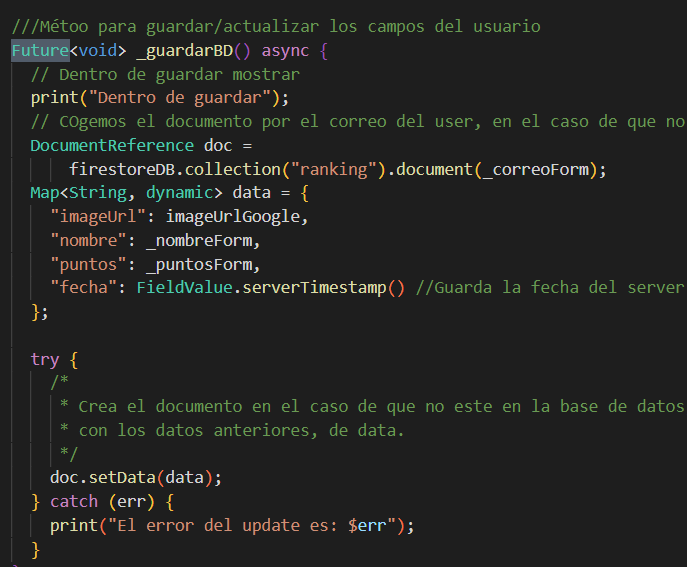
\includegraphics[width=1\textwidth]{teoria/future.png}
	\caption{Ejemplo de Future}\label{fig:future}
\end{figure}

Para ello tenemos que declarar las funciones que son asíncronas con la palabra reservada \emph{async}, de tal manera que devolverá los resultados en un tiempo x.

Cuando realicemos la llamada a estas indicaremos que se queden a la espera de respuesta con \emph{await}.

Pero podemos encontrarnos con otros objetos que también manejan tareas futuras que son los Streams. Haciendo que la aplicación de flutter sea reactiva, como es el caso del cuatro en raya o el ranking.

Estos se definen en un lugar, cogen datos de otro lugar y se queda a la escucha de que se produzcan cambios. En el caso de disparen esos cambios, el Stream se encargará de rediseñar la interfaz del usuario o de actualizar la variables, según el caso.

\section{Nuevas formas de hacer if}
Desconocía totalmente esta nueva forma de hacer los condicionales, ya que deja un código más limpio, que ocupa menos líneas e intuitivo. Un ejemplo de esto se puede ver en la imagen siguiente~\ref{fig:nuevoif}:

\begin{figure}[H]
	\centering
	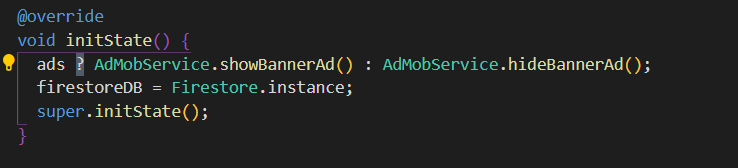
\includegraphics[width=1\textwidth]{teoria/nuevoif.png}
	\caption{Nuevas formas if}\label{fig:nuevoif}
\end{figure}

\section{Play Store}
Uno de los problemas encontrados fue a la hora de tener que generar las claves de seguridad, para que la aplicación se pueda subir a la tienda y que ciertos de los servicios estén operativos.

La incidencia estaba que no estaba generando una clave para \emph{debug} y no para \emph{release}, imposiblitando la subida.

Esto era debido a que en la documentación de Flutter siempre se realiza para el modo de test. Luego otra de las cosas a vigilar, es la ruta en la que dejamos la clave y la configuración de algunos ficheros, como los .gradle o el manifest.

Es muy importante tener la clave bien guardada porque en el caso de que se pierda, vamos a tener que volver a realizar el proceso desde cero y es algo tedioso.

\section{AdMob}
Otro de los problemas que he tenido es que a la hora de mostrar los anuncios en la aplicación, no me deja usar los que no son test. He revisado cada uno de los Ids~\ref{fig:idbanner}, pero nada.

\begin{figure}[H]
	\centering
	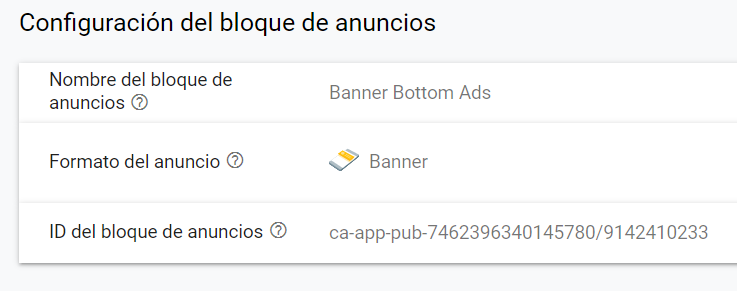
\includegraphics[width=1\textwidth]{teoria/idbanner.png}
	\caption{Banner}\label{fig:idbanner}
\end{figure}

Y las métricas de usuario si que funcionan~\ref{fig:metricas}, por lo que la instancia de adMob es la correcta.

\begin{figure}[H]
	\centering
	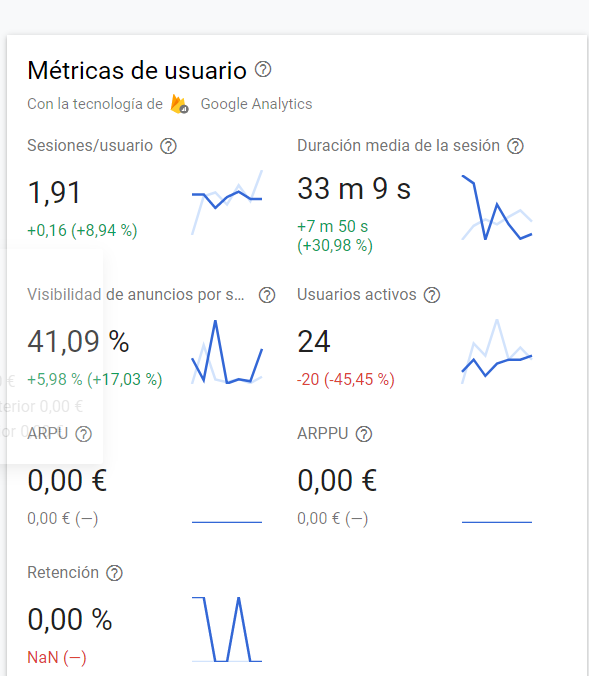
\includegraphics[height=0.8\textwidth]{teoria/metricas.png}
	\caption{Métricas usuarios}\label{fig:metricas}
\end{figure}

Tras investigar y realizar gran cantidad de pruebas creo que el problema puede estar en que no tengo métodos de cobro de ingresos. Pero es que la propia consola web de admob, no me deja introducir un método, como se puede ver en la imagen~\ref{fig:pagos}:

\begin{figure}[H]
	\centering
	
\includegraphics[width=1\textwidth]{teoria/pagos.png}
	\caption{Pagos adMob no van}\label{fig:pagos}
\end{figure}